% Copyright 2007 by Till Tantau
%
% This file may be distributed and/or modified
%
% 1. under the LaTeX Project Public License and/or
% 2. under the GNU Public License.
%
% See the file doc/licenses/LICENSE for more details.



\documentclass{beamer}

%
% DO NOT USE THIS FILE AS A TEMPLATE FOR YOUR OWN TALKS�!!
%
% Use a file in the directory solutions instead.
% They are much better suited.
%


% Setup appearance:

\usetheme{Darmstadt}
\usefonttheme[onlylarge]{structurebold}
\setbeamerfont*{frametitle}{size=\normalsize,series=\bfseries}
\setbeamertemplate{navigation symbols}{}


% Standard packages

\usepackage[english]{babel}
\usepackage[latin1]{inputenc}
\usepackage{times}
\usepackage[T1]{fontenc}
\usepackage{wasysym}
\usepackage[normalem]{ulem}               % to striketrhourhg text
\newcommand\redout{\bgroup\markoverwith
{\textcolor{red}{\rule[0.5ex]{2pt}{0.8pt}}}\ULon}
\usepackage{pdfcomment}
\usepackage{multirow}


% Setup TikZ

\usepackage{tikz}
\usetikzlibrary{arrows}
\tikzstyle{block}=[draw opacity=0.7,line width=1.4cm]
\usepackage{pgf}
\usepackage{mathrsfs}
\usepackage{appendixnumberbeamer}
\usetikzlibrary{arrows}

% Author, Title, etc.
\setbeamertemplate{footline}[frame number]
\title[]
{%
Solving Non-Linear Real Arithmetic Formulas with Virtual Substitution%
}

\author[Zaman]
{
	Author: Aklima Zaman
	\\ Supervision: Erika \'{A}brah\'{a}m
}

\institute[]
{
	Theory of Hybrid Systems - Informatik 2 - RWTH-Aachen
}

\date[WABI 2006]
{Satisfiability Checking Seminar, Winter-16/17}



% The main document

\begin{document}

\begin{frame}
	\titlepage
\end{frame}

\begin{frame}{Outline}
%%	\tableofcontents
\begin{itemize}
	\item Motivation
	\item Real Arithmetic Formula
	\item Virtual Substitution
	\begin{itemize}
		\item Sign Invariant Regions
		\item Compute Zeros
		\item Compute Test Candidates
		\item Virtual Substitution Rules
	\end{itemize}
\end{itemize}
\end{frame}

\begin{frame}{Motivation}
	\begin{itemize}
		\item \color{blue} Other related methods
			\begin{itemize}
				\item \color{green}interval constraint propagation
				\item cylindrical algebraic decomposition
			\end{itemize}
		\item \color{blue} Virtual substitution
			\begin{itemize}
				\item \color{green}applicable only to sub-language
				\item eliminates quantified variables up to degree 4
			\end{itemize}
	\end{itemize}
\end{frame}
\begin{frame}{Flow Chart of Virtual Substitution}
	\begin{center}
		\includegraphics[scale=0.28]{FlowChart-1.pdf}
	\end{center}
\end{frame}
\begin{frame}{Real Arithmetic Formula}
	\begin{itemize}
		\item <1-> Real arithmetic (RA) formula has the following syntax:\newline
		{\only<2>{\color{blue}}\textbf{polynomials:}\hspace{1mm}$t\hspace{0mm}:=\hspace{3mm}0\hspace{3mm}|\hspace{3mm}1\hspace{3mm}|\hspace{3mm}x\hspace{3mm}|\hspace{3mm}t+t\hspace{3mm}|\hspace{3mm}t - t\hspace{3mm}|\hspace{3mm}t \cdot t$\newline}
		{\only<3>{\color{blue}}\textbf{constraints:}\hspace{1mm} $c\hspace{0mm}:=\hspace{2mm}t<t$\newline}
		{\only<4>{\color{blue}}\textbf{formulas:}\hspace{5mm} $\varphi\hspace{0mm}:=\hspace{3mm}c\hspace{3mm}|\hspace{3mm}\neg\varphi\hspace{3mm}|\hspace{3mm}\varphi\wedge\varphi\hspace{3mm}|\hspace{3mm}\exists x\cdot\varphi$\newline}
		\item <5->Polynomial {\only<5>{\color{blue}}$p(x)\in Z[x_{1}\dots,x_{n}][x]$} normal form:
		{\only<5>{\color{blue}}$$ p(x) = {\only<7>{\color{blue}}a_{d}}{\only<6>{\color{blue}}x^{d}} + {\only<7>{\color{blue}}a_{d-1}}{\only<6>{\color{blue}}x^{d-1}} + \ldots + {\only<7>{\color{blue}}a_{0}}{\only<6>{\color{blue}}x^{0}} $$}
		Example:
		$$\varphi = (\underbrace{({\only<6>{\color{blue}}x^{2}}+{\only<7>{\color{blue}}2}{\only<6>{\color{blue}}x}+{\only<7>{\color{red}}4}{\only<7>{\color{red}}z})}\limits_{{\only<8>{\color{blue}}p_{1}}}\leq 0\vee \underbrace{({\only<7>{\color{blue}}y}{\only<6>{\color{blue}}x^{2}}+{\only<7>{\color{blue}}6y^{3}}{\only<6>{\color<6>{blue}}x}+{\only<7>{\color{red}}4}{\only<7>{\color{red}}z})}\limits_{{\only<8>{\color{blue}}p_{2}}}= 0)$$
	\end{itemize}
\end{frame}
\begin{frame}{Flow Chart of Virtual Substitution}
	\begin{center}
		\includegraphics[scale=0.28]{FlowChart-2.pdf}
	\end{center}
\end{frame}
\begin{frame}{Virtual Substitution}
	\begin{itemize}
		\item Quantifier elimination procedure:
		$$\exists x_{1} \dots \exists x_{n}\cdot \varphi \equiv \exists x_{1} \dots \exists x_{n-1}\cdot \psi $$
		where $\varphi, \psi$ quantifier free.
		\item <1-> Quantifier elimination by virtual substitution:
		$$\exists x_{1} \dots \exists x_{n}\cdot \varphi \equiv \exists x_{1} \dots \exists x_{n-1}\cdot \bigvee\limits_{
			{t\in T}} (\varphi[t// x]\wedge S_{t})$$
	\end{itemize}
\end{frame}
\begin{frame}{Sign Invariant Regions}
	\begin{center}
		\begin{figure}
\definecolor{xdxdff}{rgb}{0.49019607843137253,0.49019607843137253,1.}
\definecolor{uuuuuu}{rgb}{0.26666666666666666,0.26666666666666666,0.26666666666666666}
\definecolor{qqqqff}{rgb}{0.,0.,1.}
\begin{tikzpicture}[line cap=round,line join=round,>=triangle 45,x=1.0cm,y=1.0cm]
\draw[->,color=black] (-1.977740789501533,0.) -- (9.204451748455352,0.);
\foreach \x in {-1.,1.,2.,3.,4.,5.,6.,7.,8.,9.}
\draw[shift={(\x,0)},color=black] (0pt,2pt) -- (0pt,-2pt);
\draw[->,color=black] (0.,-2.876377360519662) -- (0.,2.8013630621257186);
\foreach \y in {-2.,-1.,1.,2.}
\draw[shift={(0,\y)},color=black] (2pt,0pt) -- (-2pt,0pt);
\clip(-1.977740789501533,-2.876377360519662) rectangle (9.204451748455352,2.8013630621257186);
\draw[line width=1.2pt,color=qqqqff,smooth,samples=100,domain=-1.977740789501533:9.204451748455352] plot(\x,{sin(((\x)+1.05603)*180/pi)});
\draw [line width=2.pt] (-0.8864536055584239,0.)-- (1.8960870538234125,0.);
\draw [line width=2.pt] (2.322743288261961,0.)-- (5.,0.);
\draw [line width=2.pt] (5.429913691238345,0.)-- (8.184628944026363,0.);
\draw [line width=2.pt] (-1.2300175057281486,0.)-- (-4.,0.);
\draw [line width=2.pt] (8.581504442384977,0.)-- (11.3176346026687,0.);
\draw (0.13229918803454258,2.740202483066702) node[anchor=north west] {p(x)};
\draw (8.8884554233171,-0.08337758349123406) node[anchor=north west] {x};
\begin{scriptsize}
\draw [fill=uuuuuu] (2.085562653878161,-2.8836742959461883E-10) circle (2.0pt);
\draw [fill=uuuuuu] (-1.0560300000476246,-4.7624570953530565E-11) circle (2.0pt);
\draw [fill=uuuuuu] (5.227155307181387,1.8000927273723243E-12) circle (1.5pt);
\draw [fill=uuuuuu] (8.368747960801263,-3.188346151635535E-11) circle (1.5pt);
\draw [fill=xdxdff] (-4.,0.) circle (2.5pt);
\draw[color=xdxdff] (-1.9471604999720247,2.888007215792659) node {$E$};
\draw [fill=xdxdff] (11.516767035081457,0.006426376488375775) circle (2.5pt);
\draw[color=xdxdff] (-1.9471604999720247,2.888007215792659) node {$F$};
\draw [fill=xdxdff] (-0.8864536055584239,0.) circle (1.5pt);
\draw [fill=xdxdff] (1.8960870538234125,0.) circle (1.5pt);
\draw [fill=xdxdff] (2.322743288261961,0.) circle (1.5pt);
\draw [fill=xdxdff] (5.,0.) circle (1.5pt);
\draw [fill=xdxdff] (5.429913691238345,0.) circle (1.5pt);
\draw [fill=xdxdff] (8.184628944026363,0.) circle (1.5pt);
\draw [fill=xdxdff] (-1.2300175057281486,0.) circle (1.5pt);
\draw [fill=xdxdff] (8.581504442384977,0.) circle (1.5pt);
\draw [fill=xdxdff] (11.3176346026687,0.) circle (2.5pt);
\draw[color=xdxdff] (-1.9471604999720247,2.888007215792659) node {$O$};
\end{scriptsize}
\end{tikzpicture}
\end{figure}
	\end{center}
\end{frame}
\begin{frame}{Compute Zeros}
	\only<1>{
	$p(x) = ax^{2} + bx + c$ \hspace{4mm}side condition: $a=0\wedge b=0$
	\begin{center}
		\input{constancezeros.tex}
	\end{center}
	constant polynomial $\Rightarrow$ constant zero or non zeros \newline
	
	}
	\only<2>{
	$p(x) = ax^{2} + bx + c$ \hspace{4mm} side condition: $a=0\wedge b\neq 0$
	\begin{center}
		\begin{figure}
\definecolor{qqqqff}{rgb}{0.,0.,1.}
\begin{tikzpicture}[line cap=round,line join=round,>=triangle 45,x=1.0cm,y=1.0cm]
\draw[->,color=black] (-2.805871167303091,0.) -- (7.3094000308945235,0.);
\foreach \x in {-2.5,-2.,-1.5,-1.,-0.5,0.5,1.,1.5,2.,2.5,3.,3.5,4.,4.5,5.,5.5,6.,6.5,7.}
\draw[shift={(\x,0)},color=black] (0pt,2pt) -- (0pt,-2pt);
\draw[->,color=black] (0.,-1.7750366504961292) -- (0.,3.0506791504077055);
\foreach \y in {-1.5,-1.,-0.5,0.5,1.,1.5,2.,2.5,3.}
\draw[shift={(0,\y)},color=black] (2pt,0pt) -- (-2pt,0pt);
\clip(-2.805871167303091,-1.7750366504961292) rectangle (7.3094000308945235,3.0506791504077055);
\draw [domain=-2.805871167303091:7.3094000308945235] plot(\x,{(--1.--1.*\x)/1.});
\draw (-1.6195121996132475,0.5544809744143578) node[anchor=north west] {$x$};
\draw (0.03068636446661013,3.0774391271225143) node[anchor=north west] {$p(x)$};
\draw (6.756360512121814,-0.01779817955702487) node[anchor=north west] {$x$};
\begin{scriptsize}
\draw [fill=qqqqff] (-1.,0.) circle (2.5pt);
\end{scriptsize}
\end{tikzpicture}
\end{figure}
	\end{center}
	$x = -c/b$\newline
	}
	\only<3>{
	$p(x) = ax^{2} + bx + c$ \hspace{4mm} side condition: $a\neq0\wedge b^{2}-4ac\geq 0$
	\begin{center}
		\begin{figure}
\definecolor{qqqqff}{rgb}{0.,0.,1.}
\begin{tikzpicture}[line cap=round,line join=round,>=triangle 45,x=1.0cm,y=1.0cm]
\draw[->,color=black] (-3.1381482009239074,0.) -- (3.6066083526718855,0.);
\foreach \x in {-3.,-2.5,-2.,-1.5,-1.,-0.5,0.5,1.,1.5,2.,2.5,3.,3.5}
\draw[shift={(\x,0)},color=black] (0pt,2pt) -- (0pt,-2pt);
\draw[->,color=black] (0.,-2.1344936728504944) -- (0.,1.2319368468454657);
\foreach \y in {-2.,-1.5,-1.,-0.5,0.5,1.}
\draw[shift={(0,\y)},color=black] (2pt,0pt) -- (-2pt,0pt);
\clip(-3.1381482009239074,-2.1344936728504944) rectangle (3.6066083526718855,1.2319368468454657);
\draw[line width=1.2pt,color=qqqqff,smooth,samples=100,domain=-3.1381482009239074:3.6066083526718855] plot(\x,{(\x)^(2.0)-2.0});
\draw (0.07958839122364472,1.2676233894570836) node[anchor=north west] {$p(x)$};
\draw (3.2259518981479607,0.01859439805045523) node[anchor=north west] {$x$};
\begin{scriptsize}
\draw [fill=black] (-1.4142135623730951,0.) circle (1.5pt);
\draw (-1.4142135623730951,0.) node[anchor=north west] {$x_{3}$};
\draw [fill=black] (1.4142135623730951,0.) circle (1.5pt);
\draw (1.4142135623730951,0.) node[anchor=north west] {$x_{2}$};
\end{scriptsize}
\end{tikzpicture}
\end{figure}
	\end{center}
	$x_{1} = \frac{-b - \sqrt{b^{2}-4ac}}{2a}$, $x_{2} = \frac{-b + \sqrt{b^{2}-4ac}}{2a}$\newline
}
\end{frame}
\begin{frame}{Compute Test Candidates}
	Possible solution intervals for x on $p\sim 0$:
	\begin{table}[]
		\begin{tabular}{lll}
			
\definecolor{qqqqff}{rgb}{0.,0.,1.}
\begin{tikzpicture}[line cap=round,line join=round,>=triangle 45,x=1.0cm,y=1.0cm,scale=0.3]
\draw[->,color=black] (-2.43473558731261,0.) -- (7.82390298099663,0.);
\foreach \x in {-2.,-1.5,-1.,-0.5,0.5,1.,1.5,2.,2.5,3.,3.5,4.,4.5,5.,5.5,6.,6.5,7.,7.5}
\draw[shift={(\x,0)},color=black] (0pt,2pt) -- (0pt,-2pt);
\draw[->,color=black] (0.,-2.7302059768462255) -- (0.,2.16390633079914);
\foreach \y in {-2.5,-2.,-1.5,-1.,-0.5,0.5,1.,1.5,2.}
\draw[shift={(0,\y)},color=black] (2pt,0pt) -- (-2pt,0pt);
\clip(-2.43473558731261,-2.7302059768462255) rectangle (7.82390298099663,2.16390633079914);
\draw [line width=1.2pt,color=qqqqff,domain=-2.43473558731261:7.82390298099663] plot(\x,{(--17.46-0.*\x)/17.46});
\draw [line width=1.2pt,color=qqqqff,domain=-2.43473558731261:7.82390298099663] plot(\x,{(-13.-0.*\x)/13.});
\draw [line width=1.2pt,domain=-2.43473558731261:7.82390298099663] plot(\x,{(-0.-0.*\x)/3.5});
\draw (0.09826159004769623,2.509138422367027) node[anchor=north west] {$p$};
\draw (7.082096664769683,0.010858772167722491) node[anchor=north west] {$x$};
\end{tikzpicture}
 & \input{lzros_small.tex} & \input{qzeros_small.tex}
		\end{tabular}
	\end{table}
	\begin{table}[]
		\centering
		\begin{tabular}{|c|c|c|c|c|c|c|c|}
			\hline
			Constraints & $-\infty$ & $x_{1}$ & $x_{1}+\epsilon$ & $x_{2}$ & $x_{2}+\epsilon$ & $x_{3}$ & $x_{3}+\epsilon$ \\ \hline
			$p=0$ 						& - & $\checked$ & - & $\checked$ & - & $\checked$ & - \\ \hline
			$p>0$, $p<0$, $p\neq0$ 		& $\checked$ & - & $\checked$ & - & $\checked$ & - & $\checked$ \\ \hline
			$p\geqslant0, p\leqslant0$	& $\checked$ & $\checked$ & - & $\checked$ & - & $\checked$ & - \\ \hline
		\end{tabular}
	\end{table}
\end{frame}

\begin{frame}{Example}
	\only<1,3->{
	$\varphi:=((\underbrace{xy-1}\limits_{p_{1}}=0)\wedge \underbrace{y^{2}-1}\limits_{p_{2}}<0)$\\
	Elimination of $y$:
	\begin{table}[]
		\centering
		\begin{tabular}{|c|c|c|}
			\hline
			& constraints & test candidates \\ \hline
			1. & from all constraints                & $-\infty$ \\ \hline
			2. & $p_{1}=0$                           & $1/x\hspace{.2cm}$ if $\hspace{.2cm}x \neq 0$ \\ \hline
			3. & $p_{2}<0$ & $1+\epsilon$ \\ \hline
			4. & $p_{2}<0$  & $-1+\epsilon$ \\ \hline
		\end{tabular}
	\end{table}}
\only<2>{\includegraphics[scale=0.28]{FlowChart-3.pdf}}
	\only<3->{
		\begin{table}[]
			\centering
			\begin{tabular}{llllll}
				$\exists x\cdot \exists y \cdot\varphi$  & $\leftrightarrow$ & $\exists x\cdot$ & $(\varphi[-\infty// y])$ &  & $\vee$ \\
				&  &  & $(\varphi[\dfrac{1}{x}// y]$ & $\wedge x\neq 0)$ & $\vee$ \\
				&   &   &$(\varphi[1+\epsilon// y])$ &   &$\vee$   \\
				&  &  &$(\varphi[-1+\epsilon// y])$   &   & 
			\end{tabular}
		\end{table}
	}
\end{frame}

\begin{frame}{Substitution of a Minus Infinity}

		 Assume $(p(x)=ax^{2}+bx+c )< 0$ and test candidate is $-\infty$
			\begin{table}[]
				\centering
				\begin{tabular}{llll}
					$p(x)<0[-\infty// x]$ & = & $\underbrace{{\only<1>{\color{red}}a<0}}\limits_{\only<1>{\color{blue}}\text{Case 1}}$ & $\vee$ \\
					 &  & $\underbrace{\only<2>{\color{red}}a=0 \wedge b>0}\limits_{\only<2>{\color{blue}}\text{Case 2}}$ & $\vee$ \\
					 & & $\underbrace{\only<3>{\color{red}}a=0 \wedge b=0 \wedge c<0}\limits_{\only<3>{\color{blue}}\text{Case 3}}$ &
				\end{tabular}
			\end{table}

\only<1>{\begin{figure}
\definecolor{xdxdff}{rgb}{0.49019607843137253,0.49019607843137253,1.}
\definecolor{qqqqff}{rgb}{0.,0.,1.}
\begin{tikzpicture}[line cap=round,line join=round,>=triangle 45,x=1.0cm,y=1.0cm,scale=0.7]
\draw[->,color=black] (-3.009946858088262,0.) -- (6.609896868005861,0.);
\foreach \x in {-3.,-2.5,-2.,-1.5,-1.,-0.5,0.5,1.,1.5,2.,2.5,3.,3.5,4.,4.5,5.,5.5,6.,6.5}
\draw[shift={(\x,0)},color=black] (0pt,2pt) -- (0pt,-2pt);
\draw[->,color=black] (0.,-1.412593771435594) -- (0.,3.388844984269237);
\foreach \y in {-1.,-0.5,0.5,1.,1.5,2.,2.5,3.}
\draw[shift={(0,\y)},color=black] (2pt,0pt) -- (-2pt,0pt);
\clip(-3.009946858088262,-1.412593771435594) rectangle (6.609896868005861,3.388844984269237);
\draw[line width=1.2pt,color=qqqqff,smooth,samples=100,domain=-3.009946858088262:6.609896868005861] plot(\x,{0-2.0*(\x)^(2.0)+3.0*(\x)+2.0});
\draw [line width=1.6pt] (2.096883761937013,0.)-- (8.,0.);
\draw [line width=1.6pt] (-0.6092274802358487,0.)-- (-5.,0.);
\draw (1,3.5) node[anchor=north west] {$p(x)={\color{red}-2}x² + 3x + 2$};
\draw (6.1263597494984845,0.03801758408653638) node[anchor=north west] {$x$};
\begin{scriptsize}
\draw [fill=xdxdff] (2.096883761937013,0.) circle (2.5pt);
\draw [fill=xdxdff] (8.,0.) circle (2.5pt);
\draw [fill=xdxdff] (-0.6092274802358487,0.) circle (2.5pt);
\draw [fill=xdxdff] (-5.,0.) circle (2.5pt);
\end{scriptsize}
\end{tikzpicture}
\end{figure}
}
\only<2>{\begin{figure}
\definecolor{xdxdff}{rgb}{0.49019607843137253,0.49019607843137253,1.}
\definecolor{qqqqff}{rgb}{0.,0.,1.}
\begin{tikzpicture}[line cap=round,line join=round,>=triangle 45,x=1.0cm,y=1.0cm, scale=0.7]
\draw[->,color=black] (-3.009946858088262,0.) -- (6.609896868005861,0.);
\foreach \x in {-3.,-2.5,-2.,-1.5,-1.,-0.5,0.5,1.,1.5,2.,2.5,3.,3.5,4.,4.5,5.,5.5,6.,6.5}
\draw[shift={(\x,0)},color=black] (0pt,2pt) -- (0pt,-2pt);
\draw[->,color=black] (0.,-1.412593771435594) -- (0.,3.388844984269237);
\foreach \y in {-1.,-0.5,0.5,1.,1.5,2.,2.5,3.}
\draw[shift={(0,\y)},color=black] (2pt,0pt) -- (-2pt,0pt);
\clip(-3.009946858088262,-1.412593771435594) rectangle (6.609896868005861,3.388844984269237);
\draw[line width=1.2pt,color=qqqqff,smooth,samples=100,domain=-3.009946858088262:6.609896868005861] plot(\x,{3.0*(\x)+2.0});
\draw [line width=1.6pt] (-0.8806869151873584,0.)-- (-5.,0.);
\draw (6.1263597494984845,0.03801758408653638) node[anchor=north west] {$x$};
\draw (0.0164166326631132,2.1672775269874425) node[anchor=north west] {$p(x) = {\color{red}3}x + 2$};
\begin{scriptsize}
\draw [fill=xdxdff] (8.,0.) circle (2.5pt);
\draw [fill=xdxdff] (-0.8806869151873584,0.) circle (2.5pt);
\draw [fill=xdxdff] (-5.,0.) circle (2.5pt);
\end{scriptsize}
\end{tikzpicture}
\end{figure}
}
\visible<3>{\begin{figure}
\definecolor{xdxdff}{rgb}{0.49019607843137253,0.49019607843137253,1.}
\definecolor{qqqqff}{rgb}{0.,0.,1.}
\begin{tikzpicture}[line cap=round,line join=round,>=triangle 45,x=1.0cm,y=1.0cm,scale=0.8]
\draw[->,color=black] (-2.4482985243671904,0.) -- (6.86175049877948,0.);
\foreach \x in {-2.,-1.5,-1.,-0.5,0.5,1.,1.5,2.,2.5,3.,3.5,4.,4.5,5.,5.5,6.,6.5}
\draw[shift={(\x,0)},color=black] (0pt,2pt) -- (0pt,-2pt);
\draw[->,color=black] (0.,-2.651254415953902) -- (0.,1.995560175845951);
\foreach \y in {-2.5,-2.,-1.5,-1.,-0.5,0.5,1.,1.5}
\draw[shift={(0,\y)},color=black] (2pt,0pt) -- (-2pt,0pt);
\clip(-2.4482985243671904,-2.651254415953902) rectangle (6.86175049877948,1.995560175845951);
\draw[line width=1.2pt,color=qqqqff,smooth,samples=100,domain=-2.4482985243671904:6.86175049877948] plot(\x,{0-2.0});
\draw [line width=1.6pt] (13.,0.)-- (-5.,0.);
\draw (6.122857719164664,0.033389349979935416) node[anchor=north west] {$x$};
\draw (0.12961628451116447,1.7821022617350035) node[anchor=north west] {$p(x)=\color{red}-2$};
\begin{scriptsize}
\draw [fill=xdxdff] (13.,0.) circle (2.5pt);
\draw [fill=xdxdff] (-5.,0.) circle (2.5pt);
\end{scriptsize}
\end{tikzpicture}
\end{figure}
}
\end{frame}
\begin{frame}{Example}
$\exists x \cdot \exists y \cdot ((xy-1=0)\wedge y^{2}-1<0)$
{\color{cyan}
 \begin{table}[]
 	\begin{tabular}{lllll}
 		$p(x)<0[-\infty// x]$& $=$  & $(a<0)$ & $\vee$ &$(a=0\wedge b>0)$  \\
 		&  &  &$\vee$ & $(a=0\wedge b>0\wedge c<0)$
 	\end{tabular}
 \end{table}
}
 Elimination of $y$: \hspace{2mm} Test candidate: $-\infty$
	\begin{table}[]
		\centering
		\begin{tabular}{llll}
			$\hspace{4mm}\exists x \cdot$  & $($ & \color{blue}$(xy-1=0)[-\infty//y]$ & \\ \\
			& $\wedge$ & {\color{red}$(y^{2}-1<0)[-\infty//y]$} $)$&  \\ \\
			\visible<2->{$\Leftrightarrow\exists x \cdot$  & $($ & \color{blue}$(x=0$ $\wedge -1 = 0)$ &  \\ \\}
			\visible<3->{& $\wedge$ &{\color{red}
					\begin{tabular}{lll}
					$(1<0$	& $\vee$ &$(1=0 \wedge 0>0)$  \\
						&$\vee$  & $(1=0\wedge 0=0 \wedge -1<0))$\color{black})$$
					\end{tabular}
					%$(1<0\vee(1=0 \wedge 0>0)\vee(1=0\wedge 0=0 \wedge -1<0))$
				} & \\ \\}
			\visible<4->{$\Leftrightarrow\exists x \cdot$  &  &$(\mathbf{false})$ &  \\ \\}
		\end{tabular}
	\end{table}
\end{frame}
\begin{frame}{Example: Search Tree}
	$\varphi:=((\underbrace{xy-1}\limits_{p_{1}}=0)\wedge \underbrace{y^{2}-1}\limits_{p_{2}}<0)$
	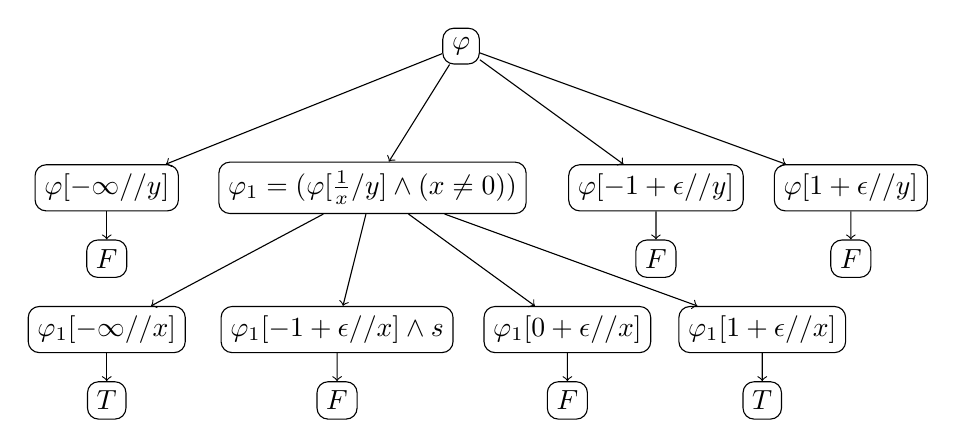
\begin{tikzpicture}[scale=0.9, 
				    state/.style={draw, rounded corners, fill=none,
				    			  text centered, text=black}]
	\node[state] (u1) at (5, 7) {$\varphi$};
	\node[state] (u2) at (0, 5) {$\varphi[-\infty//y]$};
	\node[state] (u3) at (3.75, 5) {$\varphi_{1}=(\varphi[\frac{1}{x}/y]\wedge (x\neq0))$};
	\node[state] (u4) at (7.75, 5) {$\varphi[-1+\epsilon//y]$};
	\node[state] (u5) at (0, 4) {$F$};
	\node[state] (u6) at (10.5, 5) {$\varphi[1+\epsilon//y]$};
	\node[state] (u7) at (0, 3) {$\varphi_{1}[-\infty//x]$};
	\node[state] (u8) at (3.25, 3) {$\varphi_{1}[-1+\epsilon//x] \wedge s$};
	\node[state] (u9) at (6.5, 3) {$\varphi_{1}[0+\epsilon//x]$};
	\node[state] (u15) at (9.25, 3) {$\varphi_{1}[1+\epsilon//x]$};
	\node[state] (u10) at (7.75, 4) {$F$};
	\node[state] (u11) at (10.5, 4) {$F$};
	\node[state] (u12) at (0, 2) {$T$};
	\node[state] (u13) at (3.25, 2) {$F$};
	\node[state] (u14) at (6.5, 2) {$F$};
	\node[state] (u16) at (9.25, 2) {$T$};
	
	\path[->] 	(u1)  edge   (u2);
	\path[->] 	(u1)  edge   (u3);
	\path[->] 	(u1)  edge   (u4);
	\path[->] 	(u1)  edge   (u6);
	\path[->] 	(u2)  edge   (u5);
	\path[->] 	(u3)  edge   (u7);
	\path[->] 	(u3)  edge   (u8);
	\path[->] 	(u3)  edge   (u9);
	\path[->] 	(u4)  edge   (u10);
	\path[->] 	(u6)  edge   (u11);
	\path[->] 	(u8)  edge   (u13);
	\path[->] 	(u7)  edge   (u12);
	\path[->] 	(u9)  edge   (u14);
	\path[->] 	(u3)  edge   (u15);
	\path[->] 	(u15)  edge   (u16);

\end{tikzpicture}

\end{frame}
\begin{frame}{Outlook}
	\begin{itemize}
		\item Implemented in \color{blue}SMT-RAT and \color{blue}Redlog
		\item Strengths:
		\begin{itemize}
			\item Better than Fourier Motzkin
			\item Efficient than cylindrical algebraic decomposition
		\end{itemize}
	\item Weaknesses:
	\begin{itemize}
		\item Unable to handle the formulas of degree > 4
		\item Incomplete
		\item Exponentially Complex
	\end{itemize}
	\end{itemize}
\end{frame}
\begin{frame}{Reference}
\begin{thebibliography}{9}
\bibitem{weispfenning} 
V. Weispfenning,
\textit{Quantifier elimination for real algebra - the quadratic case and beyond}.
Appl. Algebra Eng. Commun. Comput, 1997.

\bibitem{loss} 
R. Loss, V. Weispfenning,
\textit{Applying linear quantifier elimination}.
The computer Journal 36 (1993), pp. 450-462.
\end{thebibliography}
\end{frame}
\appendix
\section{More}
\begin{frame}{Substitution of Square Root Expression}
	\visible<1->{ A square root expression has following form:\newline
		$$ {\color{red}k=\frac{u+q\sqrt{r}}{s}} \hspace{2mm} \text{ with } u, q, r, s \text{ polynomials.}$$}
	\visible<2->{Assume, $p(x)=0$ and test candidate is $\frac{u+q\sqrt{r}}{s}$}
	\visible<2->{}
	\begin{enumerate}
		\visible<3->{
			\item<3-> $(p(x)=0)[\frac{u+q\sqrt{r}}{s}//x]$ to be computed.
			\item<4-> Transform the result to {\color{red}$\frac{u^{\prime}+q^{\prime}\sqrt{r}}{s^{\prime}}=0$} where $u^{\prime}, q^{\prime},s^{\prime}$ are polynomials.
			\item<5-> $\frac{u^{\prime}+q^{\prime}\sqrt{r}}{s^{\prime}}=0$\\
			\visible<6->{$\Longleftrightarrow u^{\prime}+q^{\prime}\sqrt{r} = 0$\\}
			\visible<7->{$\Longleftrightarrow u^{\prime}q^{\prime}\leq 0 \text{ }\wedge \text{ } \mid u^{\prime}\mid=\mid q^{\prime}\sqrt{r}\mid$}
			\visible<8->{$\Longleftrightarrow u^{\prime}q^{\prime}\leq 0 \text{ } \wedge \text{ } {u^{\prime}}^{2} - {q^{\prime}}^{2}r = 0$}
		}
	\end{enumerate}
\end{frame}
\begin{frame}{Substitution of Infinitesimal Expressions}
	
	\visible <1-> {Assume $p(x) < 0$ and test candidate is $e + \epsilon$}
	\visible <2-> {
		\begin{table}[]
			\centering
			\begin{tabular}{llll}
				$(p<0)[e+\epsilon// x]$  &= {\only<2>{\color{blue}}$\underbrace{((p<0)[e// x])}\limits_{\text{Case 1}}$} & $\vee$ &  \\
				& {\only<3>{\color{blue}}$\underbrace{((p=0)[e// x]\wedge(p^{\prime}<0)[e// x])}\limits_{\text{Case 2}}$}  & $\vee$ & \\
				&{\only<4>{\color{blue}}$\underbrace{((p=0)[e// x]\wedge(p^{\prime}=0)[e// x]\wedge (p^{\prime\prime}<0[e// x])}\limits_{\text{Case 3}} $} & $\vee$  & 
			\end{tabular}
		\end{table}
		\only<2>{\begin{figure}
\definecolor{qqqqff}{rgb}{0.,0.,1.}
\begin{tikzpicture}[line cap=round,line join=round,>=triangle 45,x=1.0cm,y=1.0cm,scale=0.37]
\draw[->,color=black] (-2.168471363392429,0.) -- (12.584619272493104,0.);
\foreach \x in {-2.,-1.,1.,2.,3.,4.,5.,6.,7.,8.,9.,10.,11.,12.}
\draw[shift={(\x,0)},color=black] (0pt,2pt) -- (0pt,-2pt);
\draw[->,color=black] (0.,-3.1400559790672617) -- (0.,3.8982350562185024);
\foreach \y in {-3.,-2.,-1.,1.,2.,3.}
\draw[shift={(0,\y)},color=black] (2pt,0pt) -- (-2pt,0pt);
\clip(-2.168471363392429,-3.1400559790672617) rectangle (12.584619272493104,3.8982350562185024);
\draw [rotate around={-49.891220728189076:(9.594297875672694,-8.045228486576265)},line width=1.6pt,color=qqqqff] (9.594297875672694,-8.045228486576265) ellipse (7.9584566410639725cm and 5.503377563211322cm);
\draw (0.09523037438894916,3.937264396525078) node[anchor=north west] {$p(x)$};
\draw (10.220345429631731,0.04734014596972948) node[anchor=north west] {$x$};
\begin{scriptsize}
\draw [fill=qqqqff] (13.297974890303022,-12.442118759909956) circle (2.5pt);
\draw [fill=qqqqff] (3.069022236526169,-4.442211425716545) circle (2.5pt);
\draw [fill=black] (7.493801250044723,0.) circle (2.5pt);
\draw[color=black] (7.588863713251441,0.2359819574515106) node {e};
\end{scriptsize}
\end{tikzpicture}
\end{figure}}
		\only<3>{\begin{figure}
	\definecolor{uuuuuu}{rgb}{0.26666666666666666,0.26666666666666666,0.26666666666666666}
	\definecolor{qqqqff}{rgb}{0.,0.,1.}
\definecolor{uuuuuu}{rgb}{0.26666666666666666,0.26666666666666666,0.26666666666666666}
\definecolor{qqqqff}{rgb}{0.,0.,1.}
\begin{tikzpicture}[line cap=round,line join=round,>=triangle 45,x=1.0cm,y=1.0cm,scale=0.55]
\draw[->,color=black] (-2.039374109627875,0.) -- (7.895011625124164,0.);
\foreach \x in {-2.,-1.5,-1.,-0.5,0.5,1.,1.5,2.,2.5,3.,3.5,4.,4.5,5.,5.5,6.,6.5,7.,7.5}
\draw[shift={(\x,0)},color=black] (0pt,2pt) -- (0pt,-2pt);
\draw[->,color=black] (0.,-2.7667390017137086) -- (0.,2.1826821559400207);
\foreach \y in {-2.5,-2.,-1.5,-1.,-0.5,0.5,1.,1.5,2.}
\draw[shift={(0,\y)},color=black] (2pt,0pt) -- (-2pt,0pt);
\clip(-2.039374109627875,-2.7667390017137086) rectangle (7.895011625124164,2.1826821559400207);
\draw [line width=1.2pt,color=qqqqff] (9.019416092133845,3.3468036264483025) circle (5.80723125747087cm);
\draw (0.05768763760064164,2.218225575384572) node[anchor=north west] {$p(x)$};
\draw (7.290773494566796,0.041191134405821846) node[anchor=north west] {$x$};
\begin{scriptsize}
\draw [fill=uuuuuu] (4.273592626839418,0.) circle (2.0pt);
\draw[color=uuuuuu] (4.331783825807914,0.54337846530890602) node {$e$};
\end{scriptsize}
\end{tikzpicture}
\end{figure}}
		\visible<4>{\begin{figure}
\definecolor{qqqqff}{rgb}{0.,0.,1.}
\definecolor{qqqqff}{rgb}{0.,0.,1.}
\begin{tikzpicture}[line cap=round,line join=round,>=triangle 45,x=1.0cm,y=1.0cm,scale=0.25]
\draw[->,color=black] (-4.3,0.) -- (18.7,0.);
\foreach \x in {-4.,-3.,-2.,-1.,1.,2.,3.,4.,5.,6.,7.,8.,9.,10.,11.,12.,13.,14.,15.,16.,17.,18.}
\draw[shift={(\x,0)},color=black] (0pt,2pt) -- (0pt,-2pt);
\draw[->,color=black] (0.,-4.84) -- (0.,6.3);
\foreach \y in {-4.,-3.,-2.,-1.,1.,2.,3.,4.,5.,6.}
\draw[shift={(0,\y)},color=black] (2pt,0pt) -- (-2pt,0pt);
\clip(-4.3,-4.84) rectangle (18.7,6.3);
\draw [line width=1.2pt,color=qqqqff] (7.86,-7.06) circle (7.028769451333569cm);
\draw (0.2,6.32) node[anchor=north west] {$p(x)$};
\draw (17.38,0.01) node[anchor=north west] {$x$};
\begin{scriptsize}
\draw [fill=qqqqff] (7.86,-7.06) circle (2.5pt);
\draw [fill=qqqqff] (13.42,-11.36) circle (2.5pt);
\draw [fill=black] (7.8004362960399245,-0.031482932711156764) circle (2.5pt);
\draw[color=black] (7.94,0.33) node {e};
\end{scriptsize}
\end{tikzpicture}
\end{figure}}}
\end{frame}
\begin{frame}{Example}
	$\exists x \cdot \exists y \cdot ((xy-1=0)\wedge y^{2}-1<0)$ \newline\newline
	Elimination of $y$: \newline\newline
	2.Test candidate: $\frac{1}{x} \hspace{2mm}if\hspace{2mm} x \neq 0$
	\begin{table}[]
		\centering
		\begin{tabular}{llll}
			$\hspace{4mm}\exists x \cdot$  & $($ & \color{blue}$(xy-1=0)[\frac{1}{x}//y]$ & \\
			& $\wedge$ & {\color{red}$(y^{2}-1<0)[\frac{1}{x}//y]$} &  \\
			& $\wedge$ & {\color{green}$x\neq 0$} $)$&  \\
			\visible<2->{$\Leftrightarrow\exists x \cdot$  & $($ & \color{blue}$(0=0)$ & \\}
			\visible<3->{& $\wedge$ & {\color{red}$((1>0)\wedge 1-x^{2}<0\vee(1<0 \wedge 1-x^{2}<0))$} &  \\}
			\visible<4->{& $\wedge$ & {\color{green}$x\neq 0$} $)$&  \\}
			\visible<5->{$\Leftrightarrow\exists x \cdot$ & $($ & {\color{red}$(1-x^{2}<0)$} &  \\ }
			\visible<5->{& $\wedge$ & {\color{green}$x\neq 0$} $)$&  \\}
		\end{tabular}
	\end{table}
\end{frame}
\begin{frame}{Example}
	$\exists x \cdot$  $($ {\only<1>{\color{red}$1-x^{2}<0$}} {\only<2->{\color{black}$\mathbf{true}$}}
	$\wedge$ \only<1-2>{{\only<2>{\color{red}}$x\neq 0$}} {\only<3>{\color{black}$\mathbf{true}$}} $)$\newline\newline
	Elimination of $x$:\newline\newline
	1. Test candidate: $-\infty$
	\begin{table}[]
		\centering
		\begin{tabular}{ll}
			\only<1>{
				& $(1-x_{2}<0)[-\infty//x]$   \\ \\
				= & $(-1<0 \vee (-1=0 \wedge 0>0)\vee(-1=0 \wedge 0=0 \wedge 1<0))$ \\ \\
				= & $\mathbf{true}$}
			\only<2->{
				& $(x\neq 0)[-\infty//x]$   \\ \\
				= & $(1 \neq 0 \vee 0 \neq 0)$ \\ \\
				= & $\mathbf{true}$}
		\end{tabular}
	\end{table}
\end{frame}
\end{document}


